
\def\problemset#1#2{
\begin{center}
\framebox{\framebox{\vspace{0.5in}
  \parbox{12cm}{\bf
    Gaurav Nanda \hfill Homework \#2\\
    Natural Language Processing \hfill #2, 2014}
  }}\vspace{0.05in}
\end{center}
}

\documentclass[11pt]{article}
\usepackage{fullpage}
\usepackage{algorithm}
\usepackage{algpseudocode}
\usepackage{hyperref}
\usepackage{footnote}
\usepackage{graphicx}

\setlength{\parindent}{0in}
\setlength{\parskip}{2mm}

%\setlength{\oddsidemargin}{-0.5cm}
%\setlength{\evensidemargin}{-0.5cm}
%\setlength{\textwidth}{18cm}

%\setlength{\topmargin}{-1.7cm}
%\setlength{\textheight}{25cm}
\begin{document}
\problemset{1}{March 1}

\section{Problem Statement}

There exist probabilistic sequence models that allow integrating uncertainty over multiple, interdependent classifications and collectively determine the most likely global assignment of Part of Speech Tags (POS). Two such standard models are Hidden Markov Model  (HMM) and Conditional Random Field (CRF).

Our task is to evaluate HMM and CRF models on various parameters including training accuracy, testing accuracy, runtime, accurate tag estimation for Out of Vocabolary(OOV) Words and addition of orthographic features. Both of these models are to be evaluated on Airline Travel Information Service (ATIS) and Wall Street Journal (WSJ) data sets.

\section {Testing Setup}

\subsection {Mallet Format Input}
Two models have been compared using Mallet's CRF and HMM implementations. To convert Pen TreeBank's raw data to Mallet format, I have implemented RawToMallet.java. For adding orthographic features to tagged output file, one can pass a feature file as input with suitable flags to include or exclude a particular feature.
\begin{verbatim}
~/:>cat features
CAPS  true
SUFFIX false
PREFIX true
HYPHEN false
START_NUMBER false

~/:>java RawToMallet atis3.pos feature_mallet_files/atis3_caps_prefix.mallet ./features
\end{verbatim}

\subsection {Handling OOV Tokens}

To estimate the count and testing accuracy of OOV Tokens, "evaluateInstanceList" function in "TokenAccuracyEvaluator.java" has been modified. During first iteration, all the training tokens are stored in a HashMap and all the test tokens are looked up in the Map to estimate the count and accuracy the OOV tokens.

\section {Experiments}

Various experiments have been performed to compare two models on various attributes. All the numbers computed for ATIS have been averaged over 10 random seeds. ATIS is using 80\% of the input data for training and WSJ is using 50\% data for training. WSJ (00 and 01) signifies data from 00 and 01 sections of WSJ. Similarly, WSJ (00, 01, 02 and 03) signifies data from 00, 01, 02 and 03 sections of the WSJ data set.

\subsection {Overall Test Accuracy}

\begin{center}	
	\begin{table}[ht]
  	\centering
   	\begin{tabular}{| l | l | l | l | l | l |}
    	\hline
        Model & HMM & CRF & Total TokenCount \\ \hline
        ATIS & 0.8608 & 0.9216 &  3283 \\ \hline
        WSJ (00 and 01) & 0.7859 & 0.8066 & 73576 \\ \hline
	WSJ (00, 01, 02 and 03) & 0.8324 & 0.8423 & 155513 \\ \hline
    	\end{tabular}
    	\caption{Overall Test Accuracy HMM vs CRF. }
    	\end{table}%
\end{center}

{\bfseries Analysis}

1. CRF model performs better than HMM model.

In general, generative models have to make strict independence assumptions on observations to achive tractability which reduces performance. For HMM model, this independence assumption is relaxed by arranging the output variables in a linear chain. But still to come up with a tractable model, it assumes that  state depends only on its immediate predecessor, that is, each state y$_t$ is independent of all its ancestors y$_1$, y$_2$, . . . , y$_{t-2}$ given its previous state y$_{t-1}$. Second, an HMM assumes that each observation variable x$_t$ depends only on the current state y$_t$. CRF does not make such assumptions and is a conditional probabilistic model.

Therefore, because of these assumptions, HMM does not perform as good as CRF model.

2. For WSJ corpus, testing accuracy keeps on increasing as we keep on increasing token count. With the addition of more data, models are better trained and perform better for test data. 

3. In the case of ATIS, data is restricted to a limited domain, hence not diverse. Therefore, testing accuracy is high for both HMM and CRF. I performed another experiment, where even if we use only 20\% of the data for training and rest for testing, we still get accuracy as high as 0.863.

\subsection {Test accuracy for OOV items}
\begin{center}	
	\begin{table}[ht]
  	\centering
   	\begin{tabular}{| l | l | l | l | l | l | l |}
    	\hline
        Model & HMM & CRF & OOV Count & Testing Token Count \\ \hline
        ATIS & 0.2680 & 0.3058 &  25 & 641 \\ \hline
        WSJ (00 and 01) & 0.3819 & 0.4760 & 5735 & 37465 \\ \hline
	WSJ (00, 01, 02 and 03) & 0.3938 & 0.5017 & 9340 & 81939 \\ \hline
    	\end{tabular}
    	\caption{OOV Test Accuracy HMM vs CRF. }
    	\end{table}%
\end{center}

{\bfseries Analysis}

As expected, test accuracy for OOV is very less in comparison to the seen tokens. Because these tokens were not present during training, their observation probabilities would be very less (Primarily dependent upon smoothing techniques used). However, CRF being a discriminative model still performs better than the HMM.

\subsection {Training Accuracy}

\begin{center}	
	\begin{table}[ht]
  	\centering
   	\begin{tabular}{| l | l | l | l | l | l |}
    	\hline
        Model & HMM & CRF & Total TokenCount \\ \hline
        ATIS & 0.8886 & 0.9990 &  3283 \\ \hline
        WSJ (00 and 01) & 0.8627 & 0.9953 & 73576 \\ \hline
	WSJ (00, 01, 02 and 03) & 0.8877 & 0.9936 & 155513 \\ \hline
    	\end{tabular}
    	\caption{Training Accuracy HMM vs CRF. }
    	\end{table}%
\end{center}

{\bfseries Analysis}

Training accuracy for CRF is much higher than HMM models. This is expected because CRF model uses L-BFGS optimization procedure to maximize the conditional log likelihood of the supervised training data. At the same time, CRF is more likely to overfit the training data also. This is the reason that training accuracy for ATIS is very high.

\subsection {Run Time}

There is no restriction on the number of iterations for these results (By default, CRF tagger runs for 500 iterations). However, CRF generally converged between 120-160 iterations.

\begin{center}	
	\begin{table}[ht]
  	\centering
   	\begin{tabular}{| l | l | l | l | l |}
    	\hline
        Model & HMM (sec) & CRF (sec) & Training Tokens \\ \hline
        ATIS & 5 & 57 & 2642\\ \hline
        WSJ (00 and 01) & 167 & 13100 & 36111 \\ \hline
	WSJ (00, 01, 02 and 03) & 609 & 41150 & 73574 \\ \hline
    	\end{tabular}
    	\caption{Run Time HMM vs CRF. }
    	\end{table}%
\end{center}
{\bfseries Analysis}

CRF models has to perform complex optimizations to calculate its parameters. Therefore, it takes a very large of time to train CRF models. As the data keeps on growing , CRF model does not scale well. As we doubled the size of WSJ training data, run time increased four times (However, this is also dependent upon the machine resources available at that time. But still gives a fair idea of increase in run time). 

\subsection {Adding Orthographic features}

I have introduced 5 different types of orthographic features. Words that start with CAPS, List of top 80\% Suffixes and Prefixis (http://www.darke.k12.oh.us/curriculum/la/prefixes.pdf), words having hypen and words that start with a number.  

\begin{center}	
	\begin{table}[ht]
  	\centering
   	\begin{tabular}{| l | l | l | l | l | l | l |}
    	\hline
        Features & Training Accuracy & Testing Accuracy & OOV-Accuracy & RunTime (sec) \\ \hline
	CAPS & 0.9988	 & 0.9377 & 0.3209 &  96 \\ \hline
	Hyphen & 0.9987 & 0.9301 & 0.2519 & 106 \\ \hline
	Start Number & 0.9987 & 0.9301 & 0.2519 & 98 \\ \hline
	Prefix & 0.9988 & 0.9311 & 0.2726 & 106 \\ \hline
	Suffix & 0.9988 & 0.9345 & 0.3198 & 109 \\ \hline
	All Except Suffix & 0.9991 & 0.9452 & 0.4074 & 110 \\ \hline
	All Except CAPS & 0.9991 & 0.9337 & 0.2962 & 112 \\ \hline
	\textbf{All} & \textbf{0.9988} & \textbf{0.9433} & \textbf{0.4164} & \textbf{92} \\ \hline
 	\textbf{NONE} & \textbf{0.9990} & \textbf{0.9216} & \textbf{0.3058}  & \textbf{57} \\ \hline
    	\end{tabular}
    	\caption{[ATIS] Effects of orthographic features on Overall Training Accuracy, Overall Testing Accuracy, OOV Accuracy and Runtime.}
    	\end{table}%
\end{center}

\begin{center}	
	\begin{table}[ht]
  	\centering
   	\begin{tabular}{| l | l | l | l | l | l | l |}
    	\hline
        Features & Training Accuracy & Testing Accuracy & OOV-Accuracy & RunTime (sec) \\ \hline
	CAPS & 0.9953 & 0.7372  & 0.5283 & 16405 \\ \hline
	Hyphen & 0.9954 & 0.8084 & 0.4886 & 18150 \\ \hline
	Start Number & 0.9922 & 0.8030 & 0.4711 & 10009  \\ \hline
	Prefix & 0.9952 & 0.8050 & 0.4781 & 19966 \\ \hline
	\textbf{Suffix} & \textbf{0.9954} & \textbf{0.8570} & \textbf{0.6668} & \textbf{17142} \\ \hline
	All Except Suffix & 0.9949 & 0.8332 & 0.5870 & 14498 \\ \hline
	\textbf{All} & \textbf{0.9949} & \textbf{0.8861} & \textbf{0.7819} & \textbf{16726} \\ \hline
	\textbf{NONE} & \textbf{0.9953} & \textbf{0.8066} & \textbf{0.4760} & \textbf{13100} \\ \hline	
    	\end{tabular}
    	\caption{[WSJ] Effects of orthographic features on Overall Training Accuracy, Overall Testing Accuracy, OOV Accuracy and Runtime. Trained on WSJ\_00 and Tested on WSJ\_01.}
    	\end{table}%
\end{center}

\underline{\bfseries Analysis}

\textbf{Training Accuracy}

For Both ATIS and WSJ, there is hardly an change with the increase of orthographic features. Even without new features, training accuracy is more than 99.5\%.

\textbf{Testing Accuracy}

For Both ATIS and WSJ, with addition of new features, testing accuracy increased considerably. This is major advantage of the CRF that we can easily add new features to the model and increase its testing accuracy.

To determine which feature contributed most to the increase in Accuracy, tests were run by including each of the feature separately. For ATIS, CAPS and Suffix contributed the most. For WSJ, Suffix contributed the most.

\textbf{OOV Accuracy}

With the increase of features, OOV Accuracy increased by a large number. For ATIS, CAPS contributed most to the OOV Accuracy increase and Suffix contributed most for WSJ. 

\textbf{RunTime}

For a fixed number of iterations, with increase in the number of features, run time goes up. 

We have set iteration count to 500 by default. With additional features, CRF seems to converge in lesser number of iterations. For instance for WSJ with all features it took 121 iterations to converge and without addition of any feature it took 150 iterations to complete. Therefore, increase in run time due to addition of features is somewhat compensated by lesser number of iterations.

\subsection {Accuracy with Iterations}

\begin{figure}[ht!]
\centering
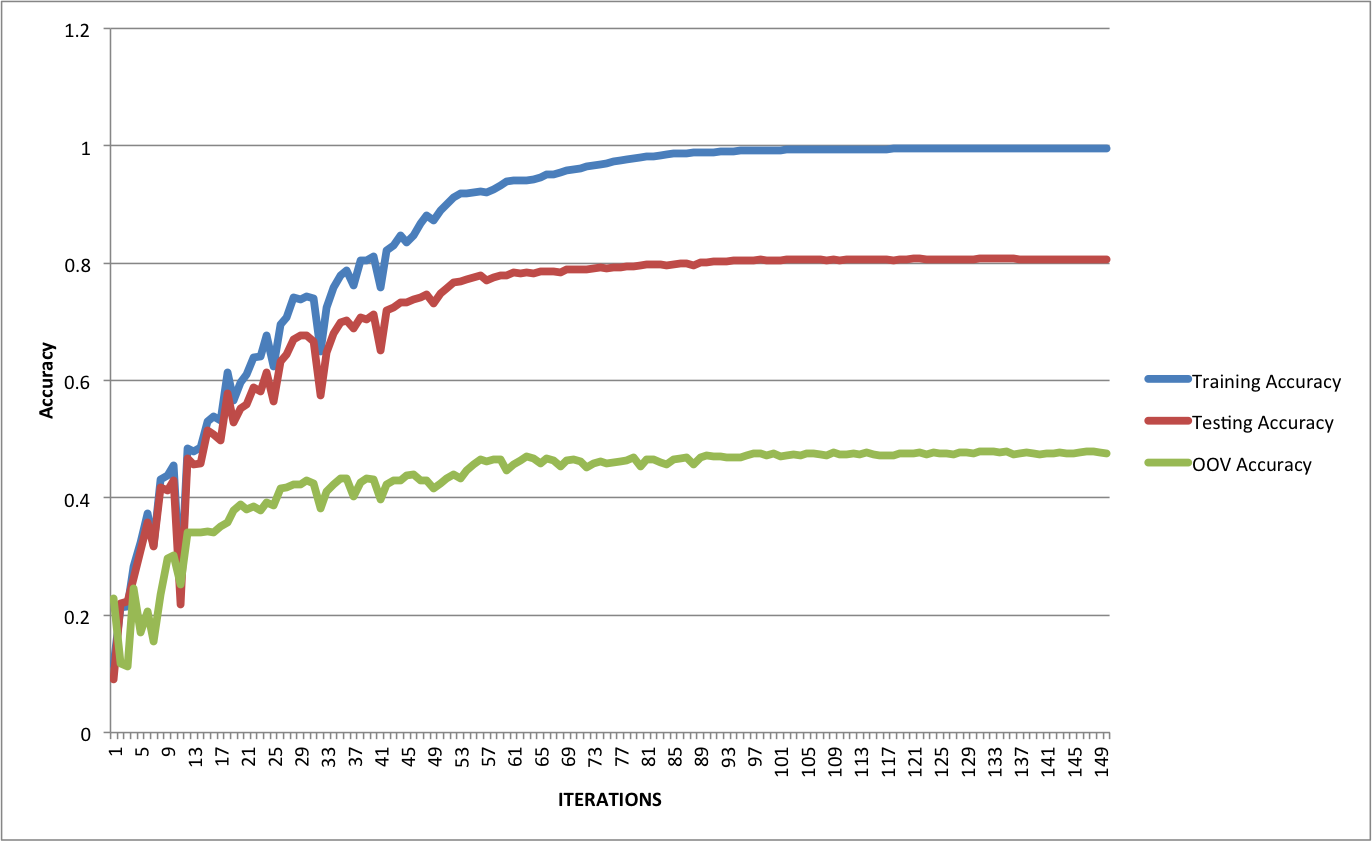
\includegraphics[width=120mm]{accuracy.png}
\caption{Accuracy with Iterations. [CRF with WSJ (00 and 01)]}
\label{accuracy}
\end{figure}

As expected for CRFs, accuracy seem to increase with addition in the number of iterations. However, percentage increase after 100 iterations is very less.

For HMMs, number of iterations hardly make any change to accuracy. On the contrary, testing accuracy for all tokens and OOV tokens is maximum with only one iteration.

\end{document}

